\chapter{Projeto - Parte 3}\label{ch:projeto-parte3}

TODO: Nesta fase do projeto, o objetivo foi criar, em \textit{python}


\section{Raciocínio Automático}\label{sec:raciocinio-automatico}

O raciocínio automático é uma área da inteligência artificial que se dedica a desenvolver algoritmos capazes de inferir conclusões a partir de um conjunto de premissas.
Pode ser visto como um processo computacional, onde se parte de uma representação de conhecimento de um determinado problema e se chega a conclusões, com base em regras de inferência (i.e., processo de manipulação de representações simbólicas para deduzir novas informações baseadas em conhecimento do domínio).

Associado ao processo de raciocínio automático, estão dois tipos de atividades principais:

\begin{enumerate}
    \item \textbf{Exploração}: A exploração das opções possíveis, e que requer antecipação e previsão das suas consequências (raciocínio prospectivo) (e.g., num determinado momento, quantas jogadas possíveis existem num jogo de xadrez para que o jogador possa ganhar o jogo)
    \item \textbf{Avaliação}: A avaliação das opções exploradas, que requer a comparação das opções possíveis e a escolha da melhor opção.
    Associadas a escolha estão métricas como o custo e a utilidade (e.g., de todas as jogadas possíveis, qual a que maximiza a probabilidade de ganhar o jogo de xadrez)
\end{enumerate}

De forma a resolver um determinado problema, através do raciocínio automático, é necessário representar o conhecimento do seu domínio através de representações simbólicas internas ao sistema - modelo do problema - com a informação necessária para a resolução do mesmo.
Estas representações servem de base à simulação para exploração e avaliação de opções possíveis, e são obtidas através de processos de codificação (i.e., da informação concreta do problema em estruturas simbólicas internas) e de descodificação (i.e., processo inverso).
A imagem~\ref{fig:representacao-problema} ilustra um exemplo de codificação e descodificação de um problema.

\begin{figure}[H]
    \begin{center}
        \resizebox{100mm}{!}{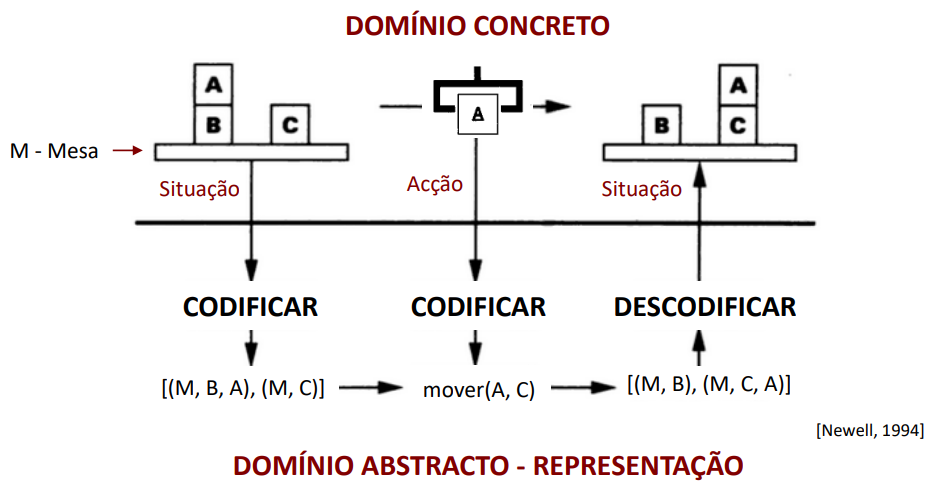
\includegraphics{../figures/representacao-problema}}
    \end{center}
    \caption{Representação de um problema.
    Retirado de~\cite{isel:iasa:slides:racicionio-automatico}, slide 8.}
    \label{fig:representacao-problema}
\end{figure}

\subsection{Modelo de um Problema}\label{subsec:modelo-problema}

O modelo de um problema é uma representação simbólica interna ao sistema, que contém a informação necessária para a resolução do problema.
O mecanismo de raciocínio automático é responsável por manipular esta representação, de forma a inferir conclusões e a resolver o problema. Esta representação tem como base os seguintes conceitos:

\begin{enumerate}
    \item \textbf{Estado}: Representação única e simbólica de um conjunto de informações concretas que caracterizam um estado da modelação de um problema. No âmbito do raciocínio automático, os estados abstraem os aspetos (configurações) estruturais que caracterizam o problema. Ao conjunto de estados possíveis de um problema e às transições entre eles, dá-se o nome de espaço de estados;
    \item \textbf{Operadores}: Representação de uma ação geradora de uma transição de um estado para outro.
    No âmbito do raciocínio automático, os operadores abstraem as transformações (dinâmicas) que ocorrem.
    Associado a um operador estão duas funções: uma que gera o estado sucessor a partir de um dado estado e outra que define o custo associado a essa transição, e que pode depender ou não do estado atual e do estado sucessor;
    \item \textbf{Transição}: Em contraste com o operador, a transição é a ação efetiva da passagem de um estado para outro (geram o estado sucessor), que ocorre quando um operador é aplicado sobre as representações internas dos estados.
    \item \textbf{Problema}: Dá suporte ao raciocínio automático, modelando um problema ao qual está inerente uma finalidade;
    Associado a um problema está o estado inicial, um conjunto de operadores e uma função predicado~\cite{stanford:fp:function-predicates} que verifica se um estado recebido é um estado objetivo ou objetivos explicítos.
    O problema considera-se resolvido quando um estado objetivo é atingido.
\end{enumerate}


\section{Mecanismo de Procura}\label{sec:mecanismo-procura}

O mecanismo de procura é um dos mecanismos de raciocínio automático, que tem como objetivo encontrar uma solução para um problema de procura.

Associado a um mecanismo de procura está o conceito de árvore de procura, que é uma estrutura responsável por manter a informação gerada durante o processo de procura.
Caracteriza-se pelos seguintes conceitos:

\begin{enumerate}
    \item \textbf{Nó}: Representa um estado do problema.
    Além disso, contém informação, tal como: operador (que foi aplicado para gerar o estado sucessor, e que pode não existir); antecessor (nó antecessor ao qual foi aplicado o operador para gerar este nó, e que pode não existir).
    E informação complementar para controlo do processo de procura: profundidade (do nó na árvore de procura, incremental a cada nível da árvore de procura); custo (associado ao caminho que vai do nó raiz ao nó, incremental a cada transição de um nó para o nó sucessor).
    Existe ainda o conceito de nós abertos (que ainda não foram expandidos) e nós fechados (que já foram expandidos);
    Os nós são comparáveis entre si através do seu custo;
    \item \textbf{Fronteira}: Representa os nós folhas da árvore de procura.
    Estes nós são candidatos a serem expandidos.
    A forma como é feita essa expansão dependerá da estratégia de procura utilizada (ver secção~\ref{sec:estrategias-procura}).
    \item \textbf{Solução}: Representa um percurso (sequência de estados e operadores), no espaço de estados, mais concretamente, corresponde ao caminho que vai do nó raiz (estado inicial) a um dos nós objetivo (estado objetivo) encontrado.
    Podem existir várias soluções para um problema de procura, que dependem também da estratégia de procura utilizada (ver secção~\ref{sec:estrategias-procura}), ou até mesmo não existir solução.
\end{enumerate}

\subsection{Processo de Procura}\label{subsec:processo-procura}

O processo de procura (ver figura~\ref{fig:processo-procura}) é um processo iterativo que tem como objetivo encontrar uma solução para um problema de procura, através da exploração do espaço de estados a partir do estado inicial.
É caracterizado, de forma abstrata, pelos seguintes passos~\cite{isel:iasa:slides:proc-espaco-estados-parte-1}:

\begin{enumerate}
    \item É criado um nó para representar o estado inicial;
    \item O nó é memorizado (depende da estratégia de procura utilizada);
    \item Enquanto a fronteira não estiver vazia
    \begin{enumerate}
        \item Remover um nó da fronteira;
        \item É verificado se o estado que lhe está associado é um estado objetivo.
        Se for um estado objetivo, o processo de procura termina, sendo devolvida a solução que contém esse nó;
        \item O nó removido é expandido, gerando os nós sucessores;
        \item Os nós sucessores são memorizados (depende da estratégia de procura utilizada).
    \end{enumerate}
    \item Se a fronteira estiver vazia, o processo de procura termina com a indicação de que não existe solução.
\end{enumerate}

\begin{figure}[H]
    \begin{center}
        \resizebox{100mm}{!}{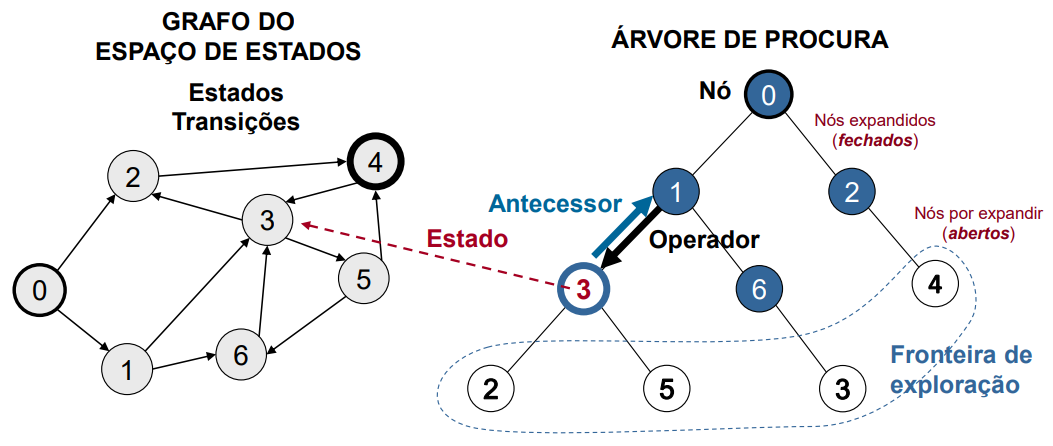
\includegraphics{../figures/processo-de-procura}}
    \end{center}
    \caption{Processo de procura.
    Retirado de~\cite{isel:iasa:slides:proc-espaco-estados-parte-1}, slide 7.}
    \label{fig:processo-procura}
\end{figure}


\section{Estratégias de Procura}\label{sec:estrategias-procura}
As estratégias de procura são responsáveis por definir a forma como a árvore de procura é explorada, ou seja, a ordem pela qual os nós são expandidos.
Existem várias estratégias de procura que se podem dividir em dois grupos: estratégias de procura não informada (cega) (ver secção~\ref{subsec:procuras-nao-informadas}) e estratégias de procura informada (heurística) (ver secção~\ref{subsec:procuras-informadas}).
Além desta divisão, existe o conceito de procura em grafo (ver secção~\ref{subsec:procura-grafo}), que é uma técnica de procura que evita estados repetidos na árvore de procura.

Alguns dos critérios de classificação das estratégias de procura são~\cite{ist:leic:resumos:procura-cega, isel:iasa:slides:proc-espaco-estados-parte-2}:

\begin{enumerate}
    \item \textbf{Completa}: Se a estratégia encontra \textbf{sempre} uma solução para o problema proposto, caso exista (e caso não exista, diz que não há solução).
    \item \textbf{Ótima}: Se a estratégia encontra a solução com o menor custo possível.
    \item \textbf{Complexidade de espaço}: Espaço de memória necessário para encontrar a solução (i.e., número máximo de nós que a estratégia mantém em memória)
    \item \textbf{Complexidade de tempo}: Tempo necessário para encontrar a solução (i.e., número de operações necessárias para encontrar a solução)
    \item \textbf{Profundidade Máxima}: Corresponde à quantidade máxima de espaços entre um qualquer par de estados ($m$), ou seja, a profundidade máxima da árvore de procura.
    \item \textbf{Fator de Ramificação}: Número máximo de sucessores de um dado nó ($b$).
    \item \textbf{Profundidade da solução}: Profundidade do nó objetivo na árvore de procura ($d$).
\end{enumerate}

\subsection{Procura em Grafo}\label{subsec:procura-grafo}

Associado a uma estratégia de procura podem se encontrar problemas de estados repetidos na árvore de procura.
Tal situação leva ao desperdício de recursos computacionais (tempo e memória), uma vez que o mesmo estado é explorado várias vezes.
A solução passa por manter uma lista de nós já explorados, que agrega os nós que já foram expandidos (nós fechados) e os nós gerados que ainda estão por expandir (nós abertos), indexada pelo estado do nó para eficiência de acesso.
No processo de geração de nós sucessores, se o nó sucessor a expandir pertencer à lista de nós
Além disso, se o nó a expandir não foi explorado, é inserido na lista de nós a explorar (nós abertos)
Baseada na procura em grafo, onde é mantida em memória uma lista de nós a explorar (fronteira) e uma lista de nós já explorados (fechados).

\subsection{Procuras Não-Informadas}\label{subsec:procuras-nao-informadas}

As procuras não-informadas (ver figura~\ref{fig:tabela-estrategias-procura-nao-informadas}) são estratégias de procura que não utilizam informação adicional para guiar o processo de procura.
Sabem apenas o que a definição do problema lhes transmite, sem qualquer tipo de pista ou heurística que permita saber se uma ação é ``mais promissora'' que outra~\cite{ist:leic:resumos:procura-cega}.

\begin{figure}[H]
    \begin{center}
        \resizebox{100mm}{!}{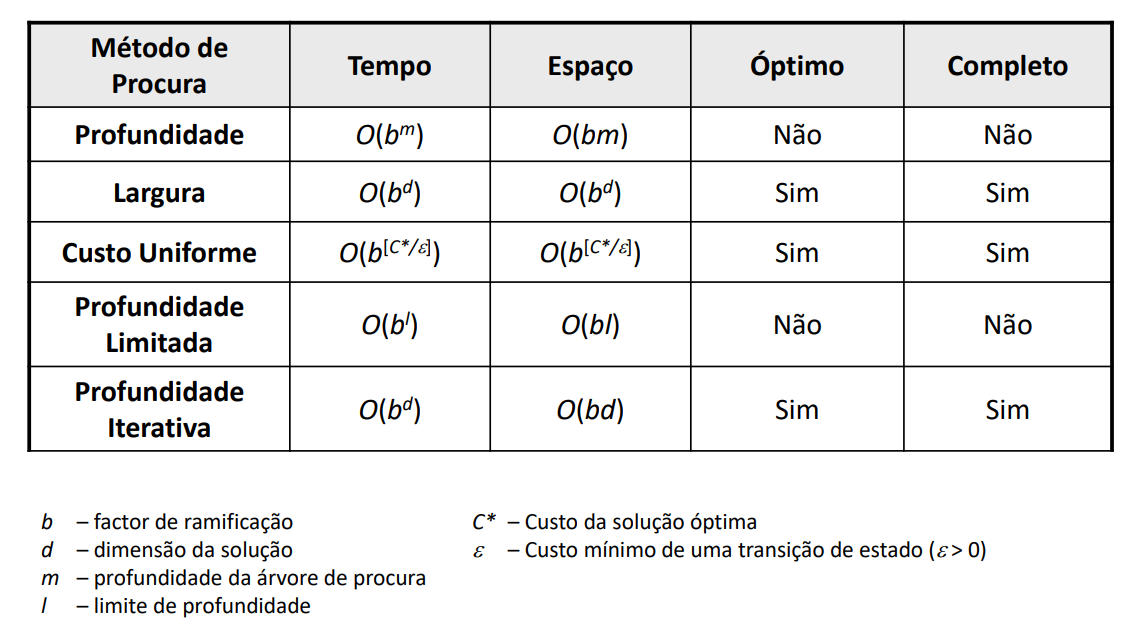
\includegraphics{../figures/tabela-estrategias-procura-nao-informadas}}
    \end{center}
    \caption{Tabela de estratégias de procura não-informadas.
    Retirado de~\cite{isel:iasa:slides:proc-espaco-estados-parte-2}, slide 12.}
    \label{fig:tabela-estrategias-procura-nao-informadas}
\end{figure}

\subsubsection{Procura em Profundidade}\label{subsubsec:procura-profundidade}

Representa um mecanismo de procura caracterizado por explorar um ramo da árvore de procura até ao fim antes de explorar outro ramo.
Utiliza uma fronteira de exploração do tipo \textit{LIFO} (Last In First Out).
Neste tipo de fronteira, os nós mais recentes são inseridos no início (de modo a serem expandidos primeiro) e a remoção é feita à cabeça.
A ordem de geração dos nós sucessores depende da ordem dos operadores aplicados~\cite{isel:iasa:slides:proc-espaco-estados-parte-1}.
Este mecanismo não garante uma solução completa (visto que podem haver profundidades infinitas ou até mesmo ciclos) e muito menos ótima (já que o primeiro nó objetivo encontrado, se existir, é o que é retornado e que não é garantidamente o melhor).

O processo de procura associado (ver figura~\ref{fig:alg-proc-profundidade}) a este mecanismo pode ser descrito pelos seguintes passos:

\begin{enumerate}
    \item Criar nó inicial a partir do estado inicial do problema;
    \item Iniciar fronteira \textit{LIFO} com o nó inicial;
    \item Enquanto a fronteira não estiver vazia:
    \begin{enumerate}
        \item Remover primeiro nó da fronteira;
        \item Verificar se estado do nó é objetivo, se for retornar solução que termina nesse nó;
        \item Expandir o nó, e para cada nó sucessor:
        \begin{enumerate}
            \item Inserir o nó na fronteira;
        \end{enumerate}
    \end{enumerate}
    \item Caso a fronteira estiver vazia, indicar que não existe solução.
\end{enumerate}

\begin{figure}[H]
    \begin{center}
        \resizebox{100mm}{!}{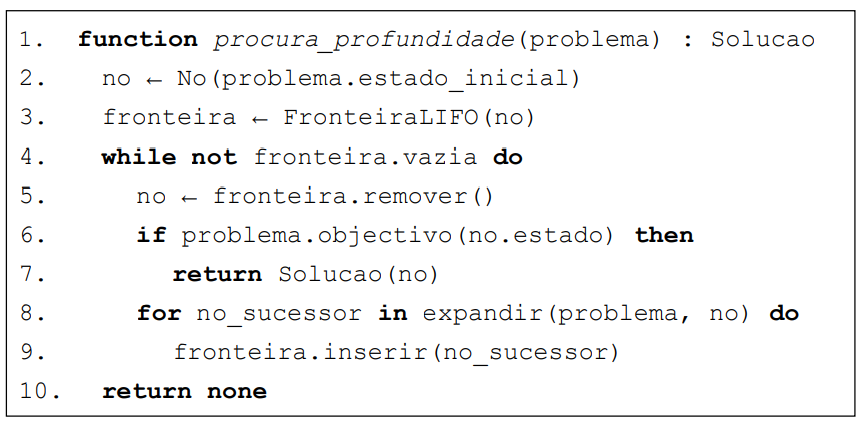
\includegraphics{../figures/alg-proc-profundidade}}
    \end{center}
    \caption{Algoritmo de procura em profundidade. Retirado de~\cite{isel:iasa:slides:proc-espaco-estados-parte-1}, slide 15.}
    \label{fig:alg-proc-profundidade}
\end{figure}

\paragraph{Procura em Profundidade Limitada}\label{par:procura-profundidade-limitada}

\paragraph{Procura em Profundidade Iterativa}\label{par:procura-profundidade-iterativa}

\subsubsection{Procura em Largura}\label{subsubsec:procura-largura}

A procura em largura é um mecanismo de procura em grafo, caracterizado por explorar todos os nós de um nível da árvore de procura antes de explorar os nós do nível seguinte.
Utiliza uma fronteira de exploração do tipo \textit{FIFO} (First In First Out).
Neste tipo de fronteira, os nós mais recentes são inseridos no fim (de modo a serem expandidos por último) e a remoção é feita ao início.

\subsubsection{Procura de Custo Uniforme}\label{subsubsec:procura-custo-uniforme}

\subsection{Procuras Informadas}\label{subsec:procuras-informadas}

Uma heurística é algo que fornece informação para resolver algo de forma expedita, são estimativas rápidas e por isso não são garantidamente ótimas (não produzem indicações robustas que garantidamente levam a boas soluções, no entanto são boas indicações e ajudam a orientar a procura).
